\chapter{Methodology}

Based on our related work, describe (using the goals outlined in the beginning) the approach I take:
creating a better model to be used in carbon-aware scheduling 
using the model and evaluating it.
\section{Improving the current Job model}

We should probably argue why the current job model used in literature is not sufficient (WaitAWhile\cite{wiesner_lets_2021} assumed constant power usage and no overhead from stopping and resuming)

\subsection{Power Measurements on Machine Learning Jobs}
\label{sec:power_measurements}

\todo{Für die Durchführung von Messungen ist es zwingend erforderlich, die verwendete Testumgebung (Hardware wie auch Software) zu dokumentieren sowie Messparameter gewissenhaft zu wählen. Zu den wichtigsten Parametern gehren die Anzahl der Messwiederholungen, die Anwendung von Warmup-Läufen sowie die Identifikation und Vermeidung möglicher störender Einflüsse.}

\todo{I feel like I should add a paragraph somewhere explaining what I want to measure}

\paragraph{Options for measuring power}

There are multiple options for measuring the power of a given computer. One way of classifying these options would be under them being either \emph{logical measurements} or \emph{physical measurements}.

Logical ones would create a model on some metrics and derive the used power. One example would be using Linux' \emph{perf} tool to read hardware performance counters. \todo{This needs some more here}

Advantages of choosing a logical approach would be that no external hardware is needed and that the overhead of the measurement would be low, as the hardware counters are being kept track of anyway. Disadvantages on the other hand would be that such a model would have to be created or chosen and would include some form of error as all models do.

Physical measurements follow another route; measurement devices would be put between the operating hardware and the power supply. The point where a power measuring device is inserted would dictate what could and could not be measured, a wall mounted measurement device could only measure all power going into a computer and not differentiate between individual programs.

Advantages of physical measurements are that they can give a more holistic measurement of a system as would be the case for a wall mounted measurement device. Portability is an issue however, unlike operating-system supported tools such as perf, a measurement device would need more effort to be used on another system (or be entirely not useable, for example when such devices are only rated for a certain power level).

Due to having a power-measurement tool on-site in our university and it allowing whole-system measurements directly, I chose to follow the physical measurement option. 

\paragraph{Measurement tool}

The concrete tool used is the \emph{Microchip MCP39F511N Power Monitor (henceforth called MCP)}, which can be inserted between the device to test and the wall mounted power supply. A picture of it can be found in figure \ref{fig:mcp}. The MCP can report the current power consumption in 10 mW steps, each 5ms.

\begin{figure}
    \missingfigure{A figure of the MCP, ask Sven about this}
    \caption[short]{The MCP}
    \label{fig:mcp}
\end{figure}

\todo{I could include an extra paragraph on why the MCP is cool, and what it does differently, perhaps. Was there anything cool? I vaguely remember some measurement devices having two capacitors to more accurately determine usage}

I then used \emph{pinpoint}, a tool for energy profiling that can use different inputs, among them being the MCP, to read out its data. 

\paragraph{The test environment}

The experiments were run on my personal computer, the components of that are listed via the \emph{hwlist} tool, with unnecessary columns and rows being redacted for brevity:

\begin{lstlisting}[language=bash, frame=single, numbers=none, caption={Hardware that was measured}, basicstyle=\ttfamily]
   $ lshw -short -C processor -C memory -C display -C bus
Class          Description
==========================
bus            AB350 Gaming K4
memory         16GiB System Memory
processor      AMD Ryzen 5 1600X Six-Core Processor
display        GP104 [GeForce GTX 1070]
\end{lstlisting}

Information about the operating system is given via \emph{hostnamectl}, again some parts redacted:

\begin{lstlisting}[language=bash, frame=single, numbers=none, caption={Used operating system information}, basicstyle=\ttfamily]
    $ hostnamectl 
   Operating System: Ubuntu 24.04 LTS                
             Kernel: Linux 6.8.0-39-generic
\end{lstlisting}

\paragraph{Measured Program}

Machine learning (ML) was used as the main motivation for checkpoint \& resume scheduling in the related works\cite {wiesner_lets_2021} and thus was also chosen by me to be measured and modeled. 

The concrete model and framework is secondary for our measurement. In my case, a small model would be chosen in order to have fewer data points for processing as well as faster iterations on the measurement script. 

There is a vast amount of machine learning frameworks. For a high-level model, the feature set of the framework only needed to support checkpointing, resuming, and some basic form of logging. 
Glancing at the documentation of popular frameworks such as \emph{torch}, \emph{tensorflow}, and \emph{huggingface} shows that these features are commonly supported. 

With not much bias towards any framework, huggingface was chosen because my supervisor Felix supplied a sample "hello-world"-esque machine learning script for python \emph{roberta.py}\footnote{\url{https://github.com/Quacck/master-thesis/blob/main/power-measurements/roberta.py}}.

The huggingface trainer supports callbacks, I thus modified the code by adding timestamped logs. These "Events" would be output into another .csv File I could later use.\todo{Later use for WHAT?!}

\paragraph{Conducted Experiments}

A script \footnote{\url{https://github.com/Quacck/master-thesis/blob/main/power-measurements/measure_roberta.sh}} was created to execute each experiment. 

On a high-level view, the following experiments were conducted: 

\begin{enumerate}
    \item \label{experiment:full}Run the whole program start to finish
    \item \label{experiment:partial_checkpointed}Run it partially, checkpointing after some step, sleeping, resuming from that step
    \item \label{experiment:partial_checkpointed_aborted}Run it partially, checkpointing after some step but aborting before the next checkpoint. Then resume as above.
    \item \label{experiment:startup_only}Run only the startup phase up until the ML would start
    \item \label{experiment:baseline}Do nothing, measure the system at rest
\end{enumerate}

Experiment \ref{experiment:full} would give a baseline for what the job would look like without checkpoint \& resume. Number \ref{experiment:partial_checkpointed} and \ref{experiment:partial_checkpointed_aborted} would be used to determine the overhead of checkpointing the job. \ref{experiment:startup_only} would be used to validate the other ones. The last experiment is necessary to determine the baseline energy consumption of the environment.

To execute these experiments inside a repeatable bash script, additional command line parameters were added to the given python script. 
For example, there would be a boolean parameter \verb|--resume_from_checkpoint|, or an integer parameter \verb|--stop_after_epoch| would be used for experiment \ref{experiment:full} to \ref{experiment:partial_checkpointed}. 
The way of doing experiment \ref{experiment:startup_only} was to copy the script, and delete everything after the imports.

\paragraph{Creating repeatable measurements}

As this is being run on standard hardware on a standard operating system, all experiment are subject to noise. 
For example, \emph{Dynamic frequency and voltage scaling (DFVS)}, the OS technique of increasing CPU "speeds" according to work load would add power in an uncontrolled way. Also, background tasks may happen "randomly", increasing power usage. 

Thus, for the testing, any foreground apps would be closed. I also used \emph{cpupower}, as shown in snippet below, to set the CPU frequency to a set value:

\todo{Think about whether this is really interesting, I guess keep it if I need more content}
\todo{What is the MAXFREQ of my ryzen 5?}
\begin{lstlisting}[language=bash, frame=single, numbers=none, caption={Used operating system information}, basicstyle=\ttfamily]
    MINFREQ=$(cpupower frequency-info --hwlimits | sed -n '1d;p' \
        | awk '{print $1}')
    MAXFREQ=$(cpupower frequency-info --hwlimits | sed -n '1d;p' \
        | awk '{print $1}')
    
    cpupower frequency-set --min ${MAXFREQ} &>/dev/null
    cpupower frequency-set --max ${MAXFREQ} &>/dev/null

    # ... conduct experiments

    cpupower frequency-set --min ${MINFREQ} &>/dev/null
    cpupower frequency-set --max ${MAXFREQ} &>/dev/null
\end{lstlisting}
\label{listing:setting_cpu_frequency}

As machine learning makes use of available GPUs, the frequency should also be similarly set to a defined value. 
NVIDIA provides guide on how to do so \footnote{\url{https://developer.nvidia.com/blog/advanced-api-performance-setstablepowerstate}}.
Sadly, my used GPU, the NVIDIA GTX 1070, is not capable of fixing the frequency as of the time of conducting these experiments. 
While it is supposed to be possible according to SOURCE\todo{Reconstruct this argument, perhaps theres still something in my PC history | grep}, but there seems to currently be drivers issue preventing this\todo{Find the forum post of people complaining}. 
Thus, the frequency of the GPU was not fixed. 
To reduce the effect of frequency scaling here, the time between experiments was increased generously so that any impact from such scaling would reoccur throughout each run and there would be reduced dependency between runs.

\todo{further explain how the experiments were conducted}

\paragraph{Conducting each experiment}

Each experiment was re-run 10 times. Between each run, there would be a \verb|sleep| period of 10 seconds and one of two minutes in the partial executions. 
Additionally, \verb|pinpoint|'s feature of measuring before and after the actual program-to-test would be used. 
This leads to a period of 30 seconds being measured around the actual experiment. 
Plotting these additional time frames would give a quick visual indicator whether experiments are sufficiently isolated from each other, ergo when the power draw is at the baseline as the actual program starts.

As there is some data being downloaded and persisted during the execution of the ML, before each run, the data would be cleaned up.

\paragraph{Collected data}

For each experiment, a named and timestamped folder would be created in the \verb|/power-measurements| folder of my repository. Each folder would then hold a \verb|.csv| with pinpoint's timestamped power measurements. 
The added timestamped-logging would be saved into another \verb|.csv|. 
While figuring out how to conduct the experiments, I would then plot these measurements early and visually spot if there were any obvious errors or mistakes.

\paragraph{Determining the baseline power draw}

Beginning with the most exiting experiment, determining the baseline and testing the amount of the underlying environment. 
One sample run is shown in Figure \ref{fig:plot_baseline}.
The blue dots in figure represent each data point. The red line is a smoothed Gaussian trend line with $\sigma = 2$. 
Dark-green vertical lines are the logged or derived "events" for each run. In this case, nothing happens, so it is only the start and end of \verb|sleep 120|. 
Notice how the trace starts 30 seconds before the start and continues for another 30 seconds because of the aforementioned \verb|pinpoint| feature.
Going further, these additional measurements will be redacted for brevity, unless something worth mentioning happens outside the actual experiments.\todo{Check later if something interesting happens or if I should reword this.}

\begin{figure}
    \includegraphics[width=\linewidth]{power-measurements/measurements_sleep_0714004033/plot.pdf}
    \caption{Sample run of the baseline experiment}
    \label{fig:plot_baseline}
\end{figure}

Across all 10 runs, the average baseline power draw is calculated via the mean of all data points. This comes out as an average of 49.8 W with a standard deviation of 4.4 W.

The baseline power draw will be less interesting going further, but will put perspective on the power draws of the other experiments. The standard deviation should give a broad idea of how much noise is in the system environment.

\paragraph{The non-interrupted run}

For the non-interrupted machine learning run, a figure of a sample run is provided in \ref{fig:plot_full}. 
Figure \ref{fig:plot_full_stacked} shows the stacked trend lines of the 10 different runs.
For simplicity's sake, I refrained from doing more elaborate statistical analysis on the different runs as the visual check of them being very similar seemed enough. 
There was an option to discuss the measurement results after normalizing each measurement point to its phase, but that would not change the result.\todo{What?}

\begin{figure}
    \includegraphics[width=\linewidth]{power-measurements/measurements_roberta_full_0714010405/plot.pdf}
    \caption{Sample run of the full run experiment}
    \label{fig:plot_full}
\end{figure}

\begin{figure}
    \includegraphics[width=\linewidth]{power-measurements/stacked_plots/roberta_full_0714.pdf}
    \caption{Stacked trend lines of the power consumption for the full runs}
    \label{fig:plot_full_stacked}
\end{figure}

The main takeaways from these measurements are:

\begin{enumerate}
    \item There is a long (about 25\%) start-up phase, which is spent in starting python, loading libraries, and loading data to disc.
    \item There are periodical work-phases; a high-power training phase would be followed by low-power evaluation\todo{Uhm, where did my evaluation phase markers go?? They are mushed together as they share a label} phase and a low-power checkpointing.
    \item There also appears to be higher variance in measurements during the training phases in comparison to the others.
\end{enumerate}

This already shows, that improvements upon the constant-power model used in \cite{wiesner_lets_2021} are possible. 
For example, in this case the start-up phase has a much lower power-draw than the work-phase.

\paragraph{Results of the checkpoint and restore experiment}

Similarly to before, results will be discussed using the stacked plots \ref{fig:plot_partial_saved_stacked} and \ref{fig:plot_partial_saved_continue_stacked}; each individual run is plotted in the repository, however.

\begin{figure}
    \includegraphics[width=\linewidth]{power-measurements/stacked_plots/roberta_stop_after_saving.pdf}
    \caption{Power draws of the ML up until stopping after epoch 2}
    \label{fig:plot_partial_saved_stacked}
\end{figure}

\begin{figure}
    \includegraphics[width=\linewidth]{power-measurements/stacked_plots/roberta_continue_after_saving.pdf}
    \caption{Power draws after continuing from the second checkpoint}
    \label{fig:plot_partial_saved_continue_stacked}
\end{figure}

Here we can observe that

\begin{enumerate}
    \item The amount of work done is the same. 
    Similarly to the full-run experiment, the ML still takes the full 5 epochs and has the same work-phases
    \item There is no overhead from checkpointing itself, as the checkpoints are being created regardless of them being resumed from later.
    \item Resuming the jobs results in an added start-up phase. This phase is slightly shorter by a few seconds than the ones in the full runs, likely due to not needing to download the dataset again.
\end{enumerate}

Additional considerations are that the amount of epoch that are worked off before checkpointing and resuming may matter, but it will be assumed that this is not the case.\todo{I could just run this again with another epoch parameter}

\paragraph{Results from checkpoint and resume with abort}

Unlike the previous experiment, where work is stopped as soon as checkpoint is created, this time the program will be stopped just before a checkpoint is created (in this case just the second checkpoint would be saved). 
This should show the maximum created overhead from a checkpoint \& resume strategy. 

While this may sound artificial, it could happen in environments where the interaction between the scheduler and the job is not well orchestrated, for example in an environment where jobs are stopped "at random" like in a cloud spot instance.\todo{Improve the wording here}.

Again, the results are visualized in figure \ref{fig:plot_partial_abort_stacked} and \ref{fig:plot_partial_abort_continue_stacked}. Attention should be paid to:

\begin{enumerate}
    \item The behavior of the repeated start-up phase is kept
    \item There is now a full additional training phase added to the overall work
\end{enumerate}

\begin{figure}
    \includegraphics[width=\linewidth]{power-measurements/stacked_plots/roberta_stop_without_saving.pdf}
    \caption{Power draws of the ML up until stopping after epoch 2}
    \label{fig:plot_partial_abort_stacked}
\end{figure}

\begin{figure}
    \includegraphics[width=\linewidth]{power-measurements/stacked_plots/roberta_continue_after_not_saving.pdf}
    \caption{Power draws after continuing from the second checkpoint}
    \label{fig:plot_partial_abort_continue_stacked}
\end{figure}

\paragraph{Calculating the energy costs of each run}

To support the argument that there is indeed an overhead from checkpointing \& resuming, I calculated the energy needed via integral of each experiment:

\begin{itemize}
    \item  unstopped costs 12.97 kJ on average with an std of 0.04
    \item  save+resume costs 13.94 kJ on average with an std of 0.1
    \item  save+abort+resume costs 15.72 kJ on average with an std of 0.07
\end{itemize}

\subsection{Defining a new model}

Now that we know what a high-level job looks like, we can pick it apart and reduce the real-world measurements of one program to a more generic model. 

Summarizing the findings from the previous paragraphs; it was shown that 

\begin{itemize}
    \item The given job has phases that have different power draws
    \item Checkpointing \& resuming carries overhead in the form of startup costs and possible wasted work.
\end{itemize}

The parameters for the improved job model are shown in form of the python implementation in \ref{listing:model_python}. \todo{Check whether this ref works}

\todo{Probably need to improve the code here}
\begin{lstlisting}[language=python, frame=single, numbers=none, caption={Python Model definition}, basicstyle=\ttfamily, label={listing:model_python}]
class Phase(TypedDict):
    name: str
    duration: float
    power: float
    is_checkpoint: NotRequired[bool]

class PhaseSpec(TypedDict):
    startup: List[Phase]
    work: List[Phase]    
\end{lstlisting}

Some simplifications are made: the duration of each phase is well known and the power per phase is a constant. Phases can also be named for later reference.
Using these specifications, a simple time-to-power function can be defined, that looks up the input time and traverses the phases in order. While not very efficient, this works well enough in a simulation environment.

The measurements that have been taken can now be fit into this new model. 
As each measurement-point can be associated to a phase via the aforementioned added logging, the average of each phase-associated measurement is used to determine the model parameters. 
The durations of the phases are calculated simularly by taking the average time the logging occured during the measurements.

Using this strategy on the 10 complete runs results in figure \ref{fig:model_overlaid}, which shows the derived model on black with the previous figure \ref{fig:plot_full} in less opacity. 
The startup phase looks well approximated, visually however there is some error during the work phases.
The training phases each have a high variance, which is not captured by the constant power approximation. After each training  phase, the power goes down seemingly liniarly, which is also approxiimated by the constant.

\todo{Should probably add the phase markers back in}
\begin{figure}
    \includegraphics[width=\linewidth]{power-measurements/model_overlaid.pdf}
    \caption{Model of roberta.py (black) vs. all measurements}
    \label{fig:model_overlaid}
\end{figure}

\paragraph{Model error analysis}

To analyse the error of this model, I cross validated the power's and total energy's RMSE using \verb|scikit-learn|'s \verb|LeaveOneOut| strategy. 
The first one would give a measure of the model's accuracy on a short-time (sub-second) scale, the latter would  tell the long-time (whole job) scale accuracy of the model.

Each of the 10 runs would be taken as the ground truth while the other 9 would be used to create the model. The results are the following: t power between the prediction and remainder has an RSME of 39.3 W while the difference in total energy is calculated as -0.1 kJ. 

Interpreting this, it seems that the model performs poorly as a predictor for die exact power used at some timepoint as the RMSE is rather large (think of the maximum power drawn being about 250W). 
However, in the context of carbon aware scheduling, this should not be too big of an issue as the time frames for carbon-emissions are order of magnitude larger. 
The high error likely comes from the high variance during the training phases which is not captured in the model.

The total energy predicted by the model is very close to the actual real life experiment, this should mean that the total carbon calculated on the model should also be close to the carbon emitted by the real program.

\begin{itemize}
    \item we can deduce phases
    \item each phase has a constant power draw
    \item give an example of how to represent the real-world measurements into a model
    \item now we should proof that the model actually represents the reality to a certain degree (error analysis)
    \item have a cute graph showing the measurements and the model-"measurements" next to each other
    \item also show that the stop-resuming functionality can be represented with our model
\end{itemize}

\section{Choosing an implementation approach}

Now that an improvement on the job model has been made, the question, on how to evaluate the implications of said model, remains. 

% We first need to explain why we chose our approach (building upon exisiting work inside GAIA). The other option that is not using a simulation would be to schedule real jobs, for example by creating a slurm plugin.

% We can then evaluate how well a slurm plugin would work for our given Forschungsragen. End that section by deeming the plugin idea as unfit, we can then shift to arguing for the simulation approach as that is also something that just came out in related work (perhaps we should see wether we list GAIA as related work or introduce it just then)

\subsection{Carbon-aware scheduling via a slurm plugin}
\label{subsec:slurm_plugin}

My first idea was to use a non-simulation approach. 
The HPI's Data Lab \footnote{\url{https://hpi.de/forschung/infrastruktur/hpi-data-engineering-lab.html}} runs a \emph{slurm} cluster and also has some nodes with power measurement infrastucture included. 
Slurm is an "open source, fault-tolerant, and highly scalable cluster management and job scheduling system for large and small Linux clusters"\footnote{\url{https://slurm.schedmd.com/overview.html}}. 
The job scheduling part is important here, it also supports a plugin infrastructure that includes scheduling plugins. 
One of the highlighted papers\cite{inigo_goiri_greenslot_2011} in the related works section specifically used slurm for its carbon-aware scheduler implementation and thus seemed like a good starting point for my own work.

\paragraph{Installing Slurm locally}

For my purposes, a local installation would suffice as I would not need to run heavy workloads but instead just the scheduling part of slurm. 
While there is a slurm \verb|apt get| package for my ubuntu version, this would not work as any plugins to be included during the slurm compilation, meaning I would have to do the same.

Slurm's documentation provides some guidelines on how to install slurm, which I followed. 
I gave cloning the main branch an attempt but I would get stuck during the compilation process, using the predefined released versions however worked.

Installing \verb|munge|\footnote{\url{https://github.com/dun/munge/wiki/Installation-Guide}} is also necessary, which is used for authentication in slurm.

One problem arose as I tried to start the \verb|slurmd|- and \verb|slurmctld| services. The first one is the worker service that would later execute jobs submitted to slurm. The latter is the main controller that, for example, schedules jobs on workers. While the command to start them would not fail, upon node inspection via Slurm's \verb|scontrol| command, it would show that all nodes are \verb|DOWN| instantly.
|
Dealing with slurm's problems usually leads to inspecting its logs, in my case the logs showed the following:

\begin{lstlisting}[language=bash, frame=single, numbers=none, caption={Slurm error logs}, basicstyle=\ttfamily]

$ less config.log

error: Couldn't find the specified plugin name for cgroup/v2
    looking at all files
error: cannot find cgroup plugin for cgroup/v2
error: cannot create cgroup context for cgroup/v2
error: Unable to initialize cgroup plugin
error: slurmd initialization failed

\end{lstlisting}

Slurm uses Linux' \verb|cgroup| feature to manage the submitted job's hardware ressources. The log hints at some problem related to slurm's usage of it.
The solution was this was to provide slurm's \verb|cgroup.conf| file. In my use-case of getting slurm to simply start, this did not need to be very sophisticated so I just used an off-the-shelf (off-the-stackoverflow\footnote{\url{https://stackoverflow.com/a/74211989}}) configuration file.

Running \verb|scontrol| again, I was finally able to see idling nodes, meaning that slurm was succesfully installed form source:

\begin{lstlisting}[language=bash, frame=single, numbers=none, caption={Slurm running}, basicstyle=\ttfamily]
$ scontrol
scontrol: update NodeName=vincent-Laptop STATE=RESUME
\end{lstlisting}

\paragraph{Creating a scheduler plugin}

The slurm documentation provides a short guide on how to add a plugin to slurm.\footnote{\url{https://slurm.schedmd.com/add.html}}. 
As a start, I simply copied slurm's default scheduler (which is also a plugin) to to the specified directory under a new name, and addings that new name to slurms build files. 
It was then was time to recompile slurm. 
Now however, during the recommended \verb|autoreconf| step, an error occured:

\begin{lstlisting}[language=bash, frame=single, numbers=none, caption={Plugin recompilation errors}, basicstyle=\ttfamily]
$ autoreconf
auxdir/x_ac_sview.m4:35: warning: macro 'AM_PATH_GLIB_2_0' 
    not found in library
configure:25140: error: possibly undefined macro: AM_PATH_GLIB_2_0
      If this token and others are legitimate, 
      please use m4_pattern_allow.
      See the Autoconf documentation.
autoreconf: error: /usr/bin/autoconf failed with exit status: 1
\end{lstlisting}

The solution, while not very obvious, was to install the \verb|libgtk2.0-dev| library. \footnote{\url{https://stackoverflow.com/questions/7805815/autoconf-error-on-ubuntu-11-04}}. 
I then added a simple logging which then showed up in slurm's log files too.

\paragraph{Adding more logic to the scheduler plugin}

One very helpful step for developing inside slurm is to enable the debugging flags.
This must be decided before compilation by using the \verb|--enable-developer| and \verb|--disable-optimizations| flags during the \verb|/configure| step. 
With that, debug symbols are added to the outgoing binaries. 
As I was using vscode, I could then attach its debugger to the running slurm thread with full functionality.

The code of the plugin runs in its own thread and there is no sandboxing or similar around it.
Thus there are seemingly no limitation on what can be done inside the plugin. 
For testing, I read out information on the incoming jobs such as set constraints or the user supplied comments. Terminating the jobs was also possible inside the plugin.

\paragraph{Problems of a scheduler plugin}

One big problem manifested in that not all jobs "showed up" inside the plugin's job queue. 
If I would submit 6 jobs, via slurm's \verb|squeue| command, only a part such as the last 3 could be logged inside the plugin.
A possible explaination for this could be slurms scheduler architecture: while there is a scheduler plugin, there also is a scheduler inside slurm's main loop. 
That main scheduler loop also uses the same job queue as the plugin.

To hack around this, I tried disabling slurm's main scheduling loop by setting \verb|sched_interval=-1| inside the slurm configuration file. 
While this had the effect of being able to access all incoming jobs inside the plugin, it also had the side-effect of disabling all logic concerning starting the jobs.
So by choosing this route, the plugin would apparently also need to re-implement alot of extra logic, which conventionally would be not be put inside the scheduler plugin. 

I also looked into whether there were any API hooks that are exposed to the plugin. 
Up until slurm version 20.11, scheduler plugins had callbacks such as when jobs were submitted. There also was support for "passive" scheduler that would get invoked when determined by slurm.
The version I tested however,  23.11, removed all such functionality and documentation. All plugins are implemented via threads that only have callbacks on when they are started and stopped.

Thus, since there was no apparent way of getting around this scheduler race condition between the plugin and the main loop. 
The scheduler approach as a whole was dropped. 
While I would not say that a plugin approach is impossible, the effort to implement one from scratch subjectivly seems very high. 
The public documentation for developing on slurm is scarce. 
There is a mailing list that can be searched, but it looks to be mostly aimed for administrating slurm and not developing it.

Other avenues that could be explored are slurm's Lua plugins. There is also a \emph{slurm simulator}\footnote{\url{https://hpckp.org/articles/how-to-use-the-slurm-simulator-as-a-development-and-testing-environment/}} which could potentially be used for carbon-aware scheduling simulation, but that I did not look into much for reasons of little documentation and seeming lack of continued support.

\subsection{Using a Simulation approach}

Thankfully, just at that time, a new paper \cite{hanafy_going_2024} was released. 
They made a prototype testbed for simulating job scheduling on cloud providers. These Jobs could be executed on spot instances (cheap VMs that seek to increase cloud utilization), on-demand instances (short-notices VMs that are thus more expensive) or pre bought VMs (medium cost, but may be wasted), the paper then discussed balancing carbon- and dollar costs. 
They included a small notion notion of hardwre requirements in the form of required CPUs per job, but that was only used to scale the cost; all hardware requirements were abstracted away in the form of the cloud always having computing ressources available.

The important part is that they also included an implementation of some schedulers used in the highlighted related works. Among that an implementation for WaitAWhile\cite{wiesner_lets_2021}.
This meant that I could add the improved job model to that exisiting testbed and have something to compare against aswell.

\paragraph{Description of the GAIA simulator}

I would first like to describe the existing testbed in detail to make it clear which part is my work and which is not.




The way to do this section would be to a) describe what was already there, and b) what I changed

\missingfigure{This would show a class diagram similar to the one in the GAIA paper, with markings which files I edited / added / deleted}

Describe the figure, explain why I am for example removing the part about the dollar-costs and the slurm-scheduler adapter. I should also describe which parts of the program I am modifiying to tackle my Forschungsfragen


Stuff I should describe about the simulation before I added anything:

\paragraph{Assumptions of the simulation}

\begin{itemize}
    \item Joblängen sind bekannt
    \item Jobs können zeitlich verschoben werden (begründet daraus, dass sie als Batch Jobs submitted werden, andere Jobs werden hierbei nicht betrachtet)
    \item User geben dabei an, wie lange der Job verschoben werden darf
    \item Die carbon curve auf dem electrical grid ist für kurze Zeiträume in der Zukunft bekannt
    \item Die Hardware ist zZ nicht begrenzt. Das war in der related work auch nicht so. Eigentlich wäre es spannend sich das anzuschauen, allerdings sind die bisherigen Scheduler halt darauf garnicht gemünzt, da werden alle Jobs unabh. voneinander gescheduled. Man könnte das via publicCloud argumentieren, allerdings wäre das questionable, in wie fern der scorelab trace benutzt werden kann (da das ja auf in einem lokalem datacenter läuft)
    \item TODO: Joblängen sollten dem Scheduler nicht bekannt sein. Die Workloads aus GAIA werden allerdings so gescheduled als ob man perfekte Knowledge hat. Das reicht zwar für ein upper bound an carbon savings, ist aber nicht sehr realistisch.  
\end{itemize}

\paragraph{Data being used}

here i could describe which data is already being used (the traces, aswell as the historical carbon data)
\begin{itemize}
    \item Welche Traces gibt es, wodurch werden die characterisiert? (Länge, Anzahl, etc, etc) Vllt. kann man hier nen coolen vergleich erstellen, Auch könnte man ein paar Sätze darüber schreiben, wie die bisher in GAIA aufgenommen wurden.
    \item Wie den scorelab trace benutzen und übersetzen? Gerne auf ner halben Seite aufschlüsseln, was die einzelnen Attribute aus sacct bedeuten.
    \item Ansonsten kann man noch die dynamic ernergy sachen als Datenquelle auflisten, bzw. das mini experiment mit fmnist und roberta 
\end{itemize}


\section{building ontop of the existing gaia sim}

Which parts of GAIA do I add on?
=> this should just be the schedulers and the part where the carbon is calculated, this ensures that 

\section{Evaluating carbon-aware scheduling with the new job model}

Hi!